\chapter{\'Equations et In\'equations}
\begin{prerequis}
Développer, factoriser par un facteur commun, résoudre une équation du premier
degré et utiliser un tableau de signes simple.
\end{prerequis}
\begin{automatismes}
Développer $(x-3)^2$; factoriser $5x^2-10x$; résoudre $3x-7=2$;
donner le signe de $(x-1)(x+4)$.
\end{automatismes}
\begin{activite}[Activité d'entrée -- Deux dimensions, même aire]
Un rectangle a pour côtés $x+2$ et $x+5$. Pour quelles valeurs de $x$ son aire
vaut-elle $28$? Mettre le problème sous forme d'équation, chercher d'abord par
essais organisés, puis transformer l'expression pour faire apparaître un trinôme.
Comparer les stratégies et discuter les contraintes géométriques sur $x$.
\end{activite}


%% ════════════════════════════════════════════════════════════════

\begin{anecdote}[Al-Khw\^{a}rizm\^{i} et la naissance de l'alg\`ebre]
En $830$, al-Khw\^{a}rizm\^{i} \'ecrivit le \textit{Kitab al-mukhtasar fi hisab
al-jabr wal-muqabala}. Il y d\'ecrivait des m\'ethodes pour r\'esoudre des \'equations
du second degr\'e --- mais uniquement en mots, sans le moindre symbole alg\'ebrique.
Il faudra attendre Fran\c{c}ois Vi\`ete ($1540$--$1603$) pour que les lettres
apparaissent en alg\`ebre.
\end{anecdote}

\begin{objectifs}
\begin{itemize}
  \item R\'esoudre les \'equations et in\'equations du second degr\'e.
  \item Factoriser $ax^2+bx+c$ gr\^ace aux racines et \`a la forme canonique.
  \item \'Etudier le signe d'un trin\^{o}me du second degr\'e.
  \item R\'esoudre des syst\`emes d'\'equations lin\'eaires.
\end{itemize}
\end{objectifs}

\section{Trin\^{o}me du second degr\'e}

\begin{defn}[Trin\^{o}me]
Un \textbf{trin\^{o}me du second degr\'e} est une expression $f(x) = ax^2+bx+c$
avec $a \ne 0$ et $a,b,c \in \R$.
\end{defn}

\begin{thm}[Discriminant]
Pour $ax^2+bx+c=0$ ($a \ne 0$), le \textbf{discriminant} est $\Delta = b^2-4ac$.
\begin{itemize}
  \item $\Delta < 0$ : aucune racine r\'eelle, $S = \emptyset$.
  \item $\Delta = 0$ : racine double $x_0 = -\dfrac{b}{2a}$,\quad
        $ax^2+bx+c = a(x-x_0)^2$.
  \item $\Delta > 0$ : deux racines
        $x_{1,2} = \dfrac{-b \pm \sqrt{\Delta}}{2a}$,\quad
        $ax^2+bx+c = a(x-x_1)(x-x_2)$.
\end{itemize}
\end{thm}

\begin{figure}[H]
\centering
\begin{tikzpicture}
\begin{axis}[width=13.2cm,height=7cm,axis lines=center,
  xlabel={$x$},ylabel={$y$},
  xmin=-4,xmax=5,ymin=-5,ymax=7,
  xtick={-3,-2,-1,0,1,2,3,4},ytick={-4,-2,0,2,4,6},
  grid=both,grid style={line width=0.2pt,draw=GM!30},
  tick label style={font=\small}]
  % parabole x^2-2x-3 : racines -1 et 3, sommet (1,-4)
  \addplot[BN,very thick,domain=-3.5:4.5,samples=120]{x^2-2*x-3};
  % sommet
  \addplot[mark=*,mark options={fill=OR,draw=OR,scale=1.5},only marks]
    coordinates{(1,-4)};
  \node[OR,font=\small,below right,fill=white,inner sep=2pt]
    at (axis cs:1,-4) {$S(\alpha,\beta)$};
  % racines
  \addplot[mark=*,mark options={fill=VE,draw=VE,scale=1.5},only marks]
    coordinates{(-1,0)(3,0)};
  \node[VE,font=\small,above left]  at (axis cs:-1,0) {$x_1$};
  \node[VE,font=\small,above right] at (axis cs:3,0)  {$x_2$};
  % axe de symétrie
  \addplot[OR!70,dashed,thick,domain=-5:7] ({1},{x});
  \node[OR!80,font=\scriptsize,anchor=west,fill=white,inner sep=1pt]
    at (axis cs:1.08,4.8) {axe $x=\alpha$};
  % annotation Delta > 0
  \node[BN,font=\small,draw=BN!30,fill=GC,rounded corners=2pt,
        inner sep=3pt] at (axis cs:-2.5,4.5)
    {$\Delta>0$, $a>0$};
  \node[BO,font=\small,fill=white,inner sep=2pt] at (axis cs:1,-1.4)
    {$f(x)<0$ entre $x_1$ et $x_2$};
\end{axis}
\end{tikzpicture}
\caption{Anatomie d'une parabole ($\Delta>0$, $a>0$).
Le sommet a pour abscisse $\alpha=-\dfrac{b}{2a}$~; les racines $x_1,x_2$ sont les z\'eros~;
$f(x)<0$ entre les racines et $f(x)>0$ en dehors.}
\end{figure}

\begin{prop}[Relations de Vi\`ete]
Si $x_1, x_2$ sont les deux racines :
$$x_1 + x_2 = -\frac{b}{a},\qquad x_1 x_2 = \frac{c}{a}.$$
\end{prop}

\begin{figure}[H]
\centering
\begin{tikzpicture}
\begin{axis}[width=13cm,height=6cm,axis lines=center,
  xlabel={$x$},ylabel={$y$},
  xmin=-3.5,xmax=4.5,ymin=-5,ymax=7,
  xtick={-3,-2,...,4},ytick={-4,-2,0,2,4,6},
  grid=both,grid style={line width=0.25pt,draw=GM!35},
  tick label style={font=\small},
  legend style={at={(0.5,-0.20)},anchor=north,legend columns=3,
                font=\scriptsize,draw=none,cells={anchor=west}}]
  \addplot[BN,thick,domain=-3.5:4.5,samples=120]{x^2-x-2};
  \addlegendentry{$x^2-x-2$\quad ($\Delta>0$)}
  \addplot[OR,thick,domain=-3.5:4.5,samples=120]{x^2-4*x+4};
  \addlegendentry{$x^2-4x+4$\quad ($\Delta=0$)}
  \addplot[BO,thick,domain=-3.5:4.5,samples=120]{x^2-2*x+3};
  \addlegendentry{$x^2-2x+3$\quad ($\Delta<0$)}
  \addplot[mark=*,mark options={fill=BN,draw=BN},only marks]
    coordinates{(-1,0)(2,0)};
  \addplot[mark=*,mark options={fill=OR,draw=OR},only marks]
    coordinates{(2,0)};
\end{axis}
\end{tikzpicture}
\caption{Trois paraboles selon le signe de $\Delta$.}
\end{figure}

\section{Signe du trin\^{o}me}

\begin{thm}[Signe]
Si $\Delta > 0$ ($x_1 < x_2$) et $a > 0$ :
\begin{center}
\begin{tikzpicture}
  \tkzTabInit[lgt=3.2,espcl=2]{$x$/1,$ax^2+bx+c$/1}
    {$-\infty$,$x_1$,$x_2$,$+\infty$}
  \tkzTabLine{,+,z,-,z,+,}
\end{tikzpicture}
\end{center}
Si $a > 0$ et $\Delta \leq 0$ : $ax^2+bx+c \geq 0$ sur tout $\R$.
\end{thm}

\section{Forme canonique}
\index{forme canonique}

\begin{methode}[Mise sous forme canonique]
Tout trin\^ome $f(x)=ax^2+bx+c$ se met sous la forme~:
$$f(x) = a\!\left(x + \frac{b}{2a}\right)^2 - \frac{\Delta}{4a},$$
o\`u $\Delta = b^2 - 4ac$. On pose $\alpha = -\dfrac{b}{2a}$ (abscisse du sommet)
et $\beta = -\dfrac{\Delta}{4a}$ (valeur au sommet).
\emph{M\'ethode pratique~:} compl\'eter le carr\'e en extrayant le coefficient
de $x^2$, puis ajouter et soustraire le bon terme.
\end{methode}

\begin{ex}[Forme canonique]
$f(x) = 2x^2 - 8x + 3$.
$$f(x) = 2(x^2 - 4x) + 3 = 2\bigl[(x-2)^2 - 4\bigr] + 3
       = 2(x-2)^2 - 5.$$
Sommet~: $(2, -5)$. Minimum de $f$~: $-5$, atteint en $x=2$.
\end{ex}

\section{Polyn\^ome de degr\'e 3}
\index{polynôme de degré 3}

\begin{defn}[Polyn\^ome de degr\'e 3]
Un \textbf{polyn\^ome de degr\'e 3} est une expression de la forme
$P(x) = ax^3 + bx^2 + cx + d$ avec $a \ne 0$.

On dit que $r$ est une \textbf{racine} de $P$ si $P(r) = 0$.
\end{defn}

\begin{thm}[Factorisation par une racine connue]
Si $r$ est une racine de $P(x) = ax^3+bx^2+cx+d$, alors il existe un
trin\^ome $Q(x) = ax^2 + ex + f$ tel que~:
$$P(x) = (x - r)\cdot Q(x).$$
On d\'etermine $Q$ par l'une des deux m\'ethodes suivantes.
\end{thm}

\begin{methode}[Identification des coefficients]
\index{identification des coefficients}
On \'ecrit $P(x) = (x-r)(ax^2+ex+f)$ et on d\'eveloppe.
En identifiant les coefficients de chaque puissance de $x$ avec ceux de $P(x)$,
on trouve $e$ et $f$.

\emph{Exemple~:} $P(x) = x^3 - 6x^2 + 11x - 6$, racine $r=1$.
$P(x) = (x-1)(x^2+ex+f)$.
D\'eveloppement~: $x^3 + ex^2 + fx - x^2 - ex - f
= x^3 + (e-1)x^2 + (f-e)x - f$.
Identification~: $e-1 = -6 \Rightarrow e=-5$~;
$-f = -6 \Rightarrow f=6$~; v\'erif~: $f-e = 6-(-5)=11$.\checkmark
Donc $P(x) = (x-1)(x^2-5x+6)$.
\end{methode}

\begin{methode}[Division euclidienne de polyn\^omes]
\index{division euclidienne!polynômes}
On divise $P(x)$ par $(x-r)$ comme une division euclidienne~:
$P(x) = (x-r)\cdot Q(x) + 0$ (le reste est nul si $r$ est racine).

\emph{Exemple~:} $P(x) = x^3 - 6x^2 + 11x - 6$ divis\'e par $(x-1)$.
\[
\begin{array}{r|l}
x^3-6x^2+11x-6 & x-1\\
\cline{2-2}
-(x^3-x^2) & x^2-5x+6\\
\cline{1-1}
\phantom{x^3{}}-5x^2+11x-6 & \\
\phantom{x^3{}}-(-5x^2+5x) & \\
\cline{1-1}
\phantom{x^3-6x^2{}}6x-6 & \\
\phantom{x^3-6x^2{}}-(6x-6) & \\
\cline{1-1}
\phantom{x^3-6x^2+11x{}}0 &
\end{array}
\]
Donc $P(x) = (x-1)(x^2-5x+6) = (x-1)(x-2)(x-3)$.
\end{methode}

\begin{prop}[Tableau de signe d'un polyn\^ome de degr\'e 3]
Si $P(x) = a(x-r_1)(x-r_2)(x-r_3)$ avec $r_1 < r_2 < r_3$ et $a>0$~:
\begin{center}
\begin{tikzpicture}
  \tkzTabInit[lgt=2.4,espcl=1.7]{$x$/1,$P(x)$/1}
    {$-\infty$,$r_1$,$r_2$,$r_3$,$+\infty$}
  \tkzTabLine{,-,z,+,z,-,z,+,}
\end{tikzpicture}
\end{center}
\end{prop}

\begin{ex}[Signe de $P(x) = (x-1)(x-2)(x-3)$]
\begin{center}
\begin{tikzpicture}
  \tkzTabInit[lgt=2.4,espcl=1.7]{$x$/1,$P(x)$/1}
    {$-\infty$,$1$,$2$,$3$,$+\infty$}
  \tkzTabLine{,-,z,+,z,-,z,+,}
\end{tikzpicture}
\end{center}
$P(x) \geq 0 \Leftrightarrow x \in [1,2]\cup[3,+\infty[$.
\end{ex}

\section{Fractions rationnelles}
\index{fraction rationnelle}

\begin{defn}[Fraction rationnelle]
Une \textbf{fraction rationnelle} est une expression de la forme
$F(x) = \dfrac{P(x)}{Q(x)}$ o\`u $P$ et $Q$ sont des polyn\^omes.
Son \textbf{ensemble de d\'efinition} est $\R \setminus \{x \mid Q(x)=0\}$.
\end{defn}

\begin{methode}[Simplifier une fraction rationnelle]
\index{simplification!fraction rationnelle}
\begin{enumerate}
  \item Factoriser num\'erateur et d\'enominateur.
  \item Simplifier les facteurs communs \emph{en notant les valeurs interdites}.
\end{enumerate}
\emph{Exemple~:} $F(x) = \dfrac{x^2-4}{x-2} = \dfrac{(x-2)(x+2)}{x-2} = x+2$
pour $x \ne 2$.
\end{methode}

\begin{methode}[\'Etudier le signe d'une fraction rationnelle]
\index{signe!fraction rationnelle}
\begin{enumerate}
  \item Factoriser $P(x)$ et $Q(x)$.
  \item Dresser le tableau de signe de chaque facteur.
  \item Conclure~: $F(x)$ a le signe du produit num./d\'en.
        (attention~: les z\'eros du d\'enominateur sont des \emph{valeurs interdites},
        pas des z\'eros de $F$).
\end{enumerate}
\end{methode}

\begin{ex}[Signe de fraction rationnelle]
$F(x) = \dfrac{(x+1)(x-3)}{x-1}$, d\'efinie sur $\R\setminus\{1\}$.
\begin{center}
\begin{tikzpicture}
  \tkzTabInit[lgt=2.3,espcl=1.45]
    {$x$/1,$x+1$/1,$x-3$/1,$x-1$/1,$F(x)$/1.1}
    {$-\infty$,$-1$,$1$,$3$,$+\infty$}
  \tkzTabLine{,-,z,+,t,+,t,+,}
  \tkzTabLine{,-,t,-,t,-,z,+,}
  \tkzTabLine{,-,t,-,z,+,t,+,}
  \tkzTabLine{,-,z,+,d,-,z,+,}
\end{tikzpicture}
\end{center}
\end{ex}

\horsprogramme{Consolidation facultative : les systèmes linéaires offrent un réinvestissement utile du calcul algébrique.}
\section{Syst\`emes d'\'equations}
\index{système d'équations}

\begin{methode}[R\'esoudre un syst\`eme $2\times 2$]
Deux m\'ethodes~:
\begin{itemize}
  \item \textbf{Substitution}~: exprimer une variable en fonction de l'autre
        et substituer.
  \item \textbf{Combinaison lin\'eaire}~: multiplier les \'equations par des
        coefficients pour faire dispara\^itre une variable.
\end{itemize}
\end{methode}

\begin{ex}[Syst\`eme par combinaison]
$\begin{cases}3x - y = 1 \\ x + 2y = 12\end{cases}$

Multiplier la premi\`ere par $2$~: $6x - 2y = 2$.
Ajouter la deuxi\`eme~: $7x = 14$, donc $x=2$.
Retour~: $y = 3\times2-1 = 5$.
\end{ex}

\section{Exercices}

\subsection*{\diff{1}\quad Niveau 1 \textemdash\ Bases et calcul direct}

\begin{exo}[R\'esoudre avec le discriminant \corrige]{1}
R\'esoudre dans $\R$ (calculer $\Delta$)~:
\begin{multicols}{2}
\begin{enumerate}
  \item $x^2 - 5x + 6 = 0$
  \item $2x^2 - 3x + 1 = 0$
  \item $x^2 + 2x + 5 = 0$
  \item $4x^2 - 12x + 9 = 0$
  \item $x^2 - 7 = 0$
  \item $3x^2 + x = 0$
  \item $x^2 - 2x - 8 = 0$
  \item $5x^2 + 3x - 2 = 0$
\end{enumerate}
\end{multicols}
\end{exo}

\begin{exo}[Forme canonique \corrige]{1}
Mettre sous forme canonique $a(x-\alpha)^2+\beta$~:
\begin{multicols}{2}
\begin{enumerate}
  \item $x^2 - 6x + 11$
  \item $2x^2 + 4x - 1$
  \item $-x^2 + 2x + 3$
  \item $x^2 + x + 1$
  \item $3x^2 - 6x + 5$
  \item $-2x^2 + 8x - 7$
\end{enumerate}
\end{multicols}
\end{exo}

\begin{exo}[In\'equations du second degr\'e \corrige]{1}
R\'esoudre et exprimer la solution en intervalle~:
\begin{multicols}{2}
\begin{enumerate}
  \item $x^2 - x - 2 \leq 0$
  \item $x^2 + 1 > 0$
  \item $-x^2 + 4x - 3 \geq 0$
  \item $2x^2 - 5x + 3 < 0$
  \item $x^2 - 4 \geq 0$
  \item $x^2 - 4x + 4 \leq 0$
\end{enumerate}
\end{multicols}
\end{exo}

\begin{exo}[Relations de Vi\`ete \corrige]{1}
\index{relations de Viète}
Sans calculer les racines, donner leur somme et leur produit~:
\begin{multicols}{2}
\begin{enumerate}
  \item $x^2 - 7x + 10$
  \item $3x^2 + x - 2$
  \item $-x^2 + 4x - 4$
  \item $x^2 - 5$
  \item $2x^2 - 6x$
  \item $x^2 - 2x + 1$
\end{enumerate}
\end{multicols}
\end{exo}

\begin{exo}[V\'erifier qu'un nombre est racine \corrige]{1}
V\'erifier que la valeur donn\'ee est bien une racine du polyn\^ome~:
\begin{enumerate}
  \item $P(x) = x^3 - 6x^2 + 11x - 6$,\quad $r = 1$
  \item $Q(x) = x^3 + 2x^2 - x - 2$,\quad $r = 1$
  \item $R(x) = 2x^3 - x^2 - 5x - 2$,\quad $r = 2$
  \item $S(x) = x^3 - 3x + 2$,\quad $r = -2$
\end{enumerate}
\end{exo}

\begin{exo}[Factoriser un polyn\^ome de degr\'e 3 \corrige]{1}
En utilisant la racine donn\'ee, factoriser compl\`etement~:
\begin{enumerate}
  \item $P(x) = x^3 - 6x^2 + 11x - 6$,\quad racine~: $r=1$
  \item $Q(x) = x^3 + 2x^2 - x - 2$,\quad racine~: $r=1$
  \item $R(x) = x^3 - 3x^2 - 4x + 12$,\quad racine~: $r=3$
  \item $S(x) = 2x^3 - x^2 - 5x - 2$,\quad racine~: $r=2$
\end{enumerate}
\end{exo}

\begin{exo}[Ensemble de d\'efinition d'une fraction rationnelle \corrige]{1}
\index{ensemble de définition}
Donner l'ensemble de d\'efinition de~:
\begin{multicols}{2}
\begin{enumerate}
  \item $\dfrac{1}{x-3}$
  \item $\dfrac{x+1}{x^2-1}$
  \item $\dfrac{x^2-4}{x^2+1}$
  \item $\dfrac{2x}{x^2-4}$
  \item $\dfrac{x-1}{(x-1)(x+2)}$
  \item $\dfrac{x^2+1}{x^2-3x+2}$
\end{enumerate}
\end{multicols}
\end{exo}

\begin{exo}[Simplifier une fraction rationnelle \corrige]{1}
Simplifier (pr\'eciser les valeurs interdites)~:
\begin{multicols}{2}
\begin{enumerate}
  \item $\dfrac{x^2-4}{x-2}$
  \item $\dfrac{x^2-1}{x+1}$
  \item $\dfrac{x^2-3x+2}{x-1}$
  \item $\dfrac{x^2+2x}{x}$
  \item $\dfrac{(x-1)^2}{x^2-1}$
  \item $\dfrac{x^3-x}{x^2-1}$
\end{enumerate}
\end{multicols}
\end{exo}

\begin{exo}[R\'esoudre un syst\`eme $2\times 2$ \corrige]{1}
R\'esoudre par substitution ou combinaison lin\'eaire~:
\begin{multicols}{2}
\begin{enumerate}
  \item $\begin{cases}2x + y = 5\\x - 3y = -1\end{cases}$
  \item $\begin{cases}3x - y = 1\\x + 2y = 12\end{cases}$
  \item $\begin{cases}x + y = 7\\2x - y = 2\end{cases}$
  \item $\begin{cases}4x - 3y = 0\\2x + y = 10\end{cases}$
\end{enumerate}
\end{multicols}
\end{exo}

\begin{exo}[Tableau de signe d'un trin\^ome \corrige]{1}
Dresser le tableau de signe et r\'esoudre l'in\'equation~:
\begin{enumerate}
  \item $x^2 - 4x + 3 > 0$
  \item $-2x^2 + x + 1 \geq 0$
  \item $x^2 - 2x + 1 \leq 0$
  \item $(2x-1)(x+3) < 0$
\end{enumerate}
\end{exo}

\begin{exo}[Construire une \'equation de solution donn\'ee \corrige]{1}
Construire l'\'equation $ax^2+bx+c=0$ (avec $a=1$) dont les racines sont~:
\begin{multicols}{2}
\begin{enumerate}
  \item $x_1=2$ et $x_2=5$
  \item $x_1=-1$ et $x_2=3$
  \item $x_1 = x_2 = 4$
  \item $x_1=\sqrt{2}$ et $x_2=-\sqrt{2}$
  \item $x_1=1+\sqrt{3}$ et $x_2=1-\sqrt{3}$
  \item $x_1=0$ et $x_2=7$
\end{enumerate}
\end{multicols}
\end{exo}

\begin{exo}[Valeur num\'erique d'un polyn\^ome \corrige]{1}
Calculer $P(-1)$, $P(0)$, $P(2)$, $P(3)$ pour~:
\begin{enumerate}
  \item $P(x) = x^3 - 3x^2 + 2x - 1$
  \item $P(x) = 2x^3 + x^2 - x + 4$
\end{enumerate}
\end{exo}

\begin{exo}[Discriminant et nombre de solutions \corrige]{1}
Sans r\'esoudre, d\'eterminer le nombre de solutions r\'eelles de chaque \'equation~:
\begin{multicols}{2}
\begin{enumerate}
  \item $3x^2 - 5x + 3 = 0$
  \item $x^2 - 6x + 9 = 0$
  \item $2x^2 + 7x - 4 = 0$
  \item $x^2 + x + 1 = 0$
  \item $4x^2 - 4x + 1 = 0$
  \item $x^2 + 2x - 15 = 0$
\end{enumerate}
\end{multicols}
\end{exo}

\begin{exo}[Lire les racines sur un graphe \corrige]{1}
Pour chacune des paraboles repr\'esent\'ees (non fournies ici, \`a tracer)~:
\begin{enumerate}
  \item $f(x) = x^2 - 4x + 3$~: tracer la parabole et lire graphiquement les racines.
  \item $g(x) = -x^2 + 2x + 3$~: tracer et lire.
  \item V\'erifier alg\'ebriquement en calculant $\Delta$.
\end{enumerate}
\end{exo}

\begin{exo}[Signe d'une fraction simple \corrige]{1}
Dresser le tableau de signe de~:
\begin{multicols}{2}
\begin{enumerate}
  \item $\dfrac{x-2}{x+1}$
  \item $\dfrac{-x+3}{x-5}$
  \item $\dfrac{x^2-1}{x}$
  \item $\dfrac{(x+2)^2}{x-4}$
\end{enumerate}
\end{multicols}
\end{exo}

\subsection*{\diff{2}\quad Niveau 2 \textemdash\ Combinaisons et applications}

\begin{exo}[Fraction rationnelle~: signe et domaine \corrige]{2}
Pour chaque fraction~: (a) donner l'ensemble de d\'efinition~; (b) dresser
le tableau de signe~; (c) r\'esoudre $F(x) > 0$.
\begin{enumerate}
  \item $F(x) = \dfrac{x^2-x-2}{x^2-4}$
  \item $F(x) = \dfrac{(x-1)(x+2)}{x^2-9}$
  \item $F(x) = \dfrac{x^2-3x}{x^2-x-6}$
  \item $F(x) = \dfrac{x^3-x}{x^2+1}$
\end{enumerate}
\end{exo}

\begin{exo}[Factoriser un polyn\^ome de degr\'e 3 compl\`etement \corrige]{2}
Sachant qu'une racine est un entier compris entre $-3$ et $3$, trouver
cette racine et factoriser compl\`etement~:
\begin{enumerate}
  \item $P(x) = x^3 - 7x + 6$
  \item $Q(x) = x^3 + x^2 - 4x - 4$
  \item $R(x) = 2x^3 - 3x^2 - 11x + 6$
  \item $S(x) = x^3 - 4x^2 + x + 6$
\end{enumerate}
\end{exo}

\begin{exo}[Tableau de signe d'un polyn\^ome de degr\'e 3 \corrige]{2}
Apr\`es factorisation, dresser le tableau de signe et r\'esoudre l'in\'equation~:
\begin{enumerate}
  \item $x^3 - 6x^2 + 11x - 6 \geq 0$ \quad(racine $r=1$)
  \item $(x-1)(x^2+x+1) > 0$
  \item $x^3 + x^2 - 4x - 4 \leq 0$ \quad(racine $r=2$)
  \item $2x^3 - x^2 - x \geq 0$
\end{enumerate}
\end{exo}

\begin{exo}[Op\'erations sur les fractions rationnelles \corrige]{2}
Simplifier ou calculer~:
\begin{multicols}{2}
\begin{enumerate}
  \item $\dfrac{x^2-1}{x+1} + \dfrac{1}{x-1}$
  \item $\dfrac{x}{x-2} - \dfrac{2}{x+1}$
  \item $\dfrac{x^2-4}{x-2} \times \dfrac{x-1}{x+2}$
  \item $\dfrac{x^2-9}{x+3} \div (x-3)$
  \item $\dfrac{1}{x} + \dfrac{1}{x+1} + \dfrac{1}{x+2}$
  \item $\left(\dfrac{x}{x+1}\right)^2 - \dfrac{x^2}{x^2-1}$
\end{enumerate}
\end{multicols}
\end{exo}

\begin{exo}[Param\`etre dans le discriminant \corrige]{2}
D\'eterminer $m$ pour que l'\'equation ait~:
\begin{enumerate}
  \item $x^2 + mx + m = 0$~: deux racines r\'eelles~; une racine double~; pas de racine.
  \item $mx^2 - 2x + 1 = 0$~: deux solutions distinctes ($m \ne 0$).
  \item $x^2 - (m+1)x + m = 0$~: une des racines vaut $1$.
  \item $x^2 + 2mx + (m+2) = 0$~: les deux racines sont positives.
\end{enumerate}
\end{exo}

\begin{exo}[Syst\`eme m\^el\'e lin\'eaire/quadratique \corrige]{2}
R\'esoudre les syst\`emes suivants~:
\begin{enumerate}
  \item $\begin{cases}y = x^2 - 2x \\ y = x + 4\end{cases}$
        (positions relatives de la parabole et de la droite)
  \item $\begin{cases}x + y = 5 \\ xy = 6\end{cases}$
        \emph{(Indication~: $x$ et $y$ sont racines d'un trin\^ome.)}
  \item $\begin{cases}x^2 + y^2 = 25 \\ y = x + 1\end{cases}$
\end{enumerate}
\end{exo}

\begin{exo}[R\'esoudre une \'equation avec fraction rationnelle \corrige]{2}
R\'esoudre dans leur domaine de d\'efinition~:
\begin{multicols}{2}
\begin{enumerate}
  \item $\dfrac{x+1}{x-1} = 2$
  \item $\dfrac{x}{x+2} + \dfrac{1}{x} = 1$
  \item $\dfrac{x^2-1}{x+1} = x-2$
  \item $\dfrac{3}{x-2} = \dfrac{x+1}{x}$
\end{enumerate}
\end{multicols}
\end{exo}

\begin{exo}[In\'egalit\'e avec fraction rationnelle \corrige]{2}
R\'esoudre dans leur domaine de d\'efinition~:
\begin{multicols}{2}
\begin{enumerate}
  \item $\dfrac{x+3}{x-2} > 1$
  \item $\dfrac{x^2-4}{x+1} \leq 0$
  \item $\dfrac{x-1}{x+1} \geq \dfrac{x+1}{x-1}$
  \item $\dfrac{1}{x} + 1 > 0$
\end{enumerate}
\end{multicols}
\end{exo}

\begin{exo}[Application~: probl\`eme de g\'eom\'etrie \corrige]{2}
\begin{enumerate}
  \item Un rectangle a un p\'erim\`etre de $20$~cm et une aire de $24$~cm$^2$.
        Trouver ses dimensions.
  \item Un terrain rectangulaire a une longueur sup\'erieure de $5$~m
        \`a sa largeur. Son aire est de $204$~m$^2$. Trouver ses dimensions.
  \item Un carr\'e et un rectangle de m\^eme aire ont respectivement
        pour c\^ot\'e $a$ et pour dimensions $(a-2)$ et $(a+3)$.
        Trouver $a$.
\end{enumerate}
\end{exo}

\begin{exo}[Division euclidienne de polyn\^omes \corrige]{2}
Effectuer la division euclidienne de $P(x)$ par $Q(x)$
et \'ecrire $P(x) = Q(x)\cdot A(x) + R$~:
\begin{enumerate}
  \item $P(x) = x^3 - 2x^2 + x - 1$ par $Q(x) = x - 1$
  \item $P(x) = 2x^3 + x^2 - 3x + 2$ par $Q(x) = x + 2$
  \item $P(x) = x^3 + x - 2$ par $Q(x) = x - 1$
\end{enumerate}
V\'erifier que le reste est bien $P(r)$ (th\'eor\`eme de B\'ezout).
\end{exo}

\begin{exo}[Factoriser ou d\'evelopper \corrige]{1}
D\'evelopper ou factoriser selon le cas~:
\begin{multicols}{2}
\begin{enumerate}
  \item $(x+3)(x-3)$
  \item $(2x-1)^2$
  \item $x^2-9$
  \item $4x^2-4x+1$
  \item $(x+2)(x^2-2x+4)$
  \item $x^3+8$
\end{enumerate}
\end{multicols}
\end{exo}

\begin{exo}[R\'esoudre avec le discriminant (suite) \corrige]{1}
R\'esoudre dans $\R$~:
\begin{multicols}{2}
\begin{enumerate}
  \item $x^2 - \sqrt{5}\,x = 0$
  \item $(x-1)(x+2)=4$
  \item $x^2 = 2x - 1$
  \item $\dfrac{x^2+1}{2} = x$
\end{enumerate}
\end{multicols}
\end{exo}

\begin{exo}[Probl\`eme de vitesse \corrige]{1}
Un train parcourt $360$~km. S'il allait $30$~km/h plus vite, il mettrait
$1$~h de moins. Trouver sa vitesse actuelle en r\'esolvant une \'equation
du second degr\'e.
\end{exo}

\begin{exo}[Signe d'un produit de facteurs \corrige]{2}
\'Etudier le signe de~:
\begin{multicols}{2}
\begin{enumerate}
  \item $x^2(x-1)$
  \item $(x+2)^2(x-3)$
  \item $\dfrac{x^2-9}{(x+1)^2}$
  \item $(x^2-4)(x^2-1)$
\end{enumerate}
\end{multicols}
\end{exo}

\begin{exo}[Valeurs interdites et simplification \corrige]{2}
Pour chaque expression, donner les valeurs interdites de $x$,
simplifier et donner le domaine~:
\begin{multicols}{2}
\begin{enumerate}
  \item $\dfrac{x^2-x}{x-1}$
  \item $\dfrac{x^3-4x}{x^2-4}$
  \item $\dfrac{x^2+3x+2}{x^2-1}$
  \item $\dfrac{x^3+x^2}{x^2+x}$
\end{enumerate}
\end{multicols}
\end{exo}

\begin{exo}[\logicoalgo\ Algorithme~: r\'esoudre $ax^2+bx+c=0$ \corrige]{2}

\begin{algorithm}[H]
\caption{R\'esolution de l'\'equation du second degr\'e}
\KwIn{trois r\'eels $a\ne0$, $b$, $c$}
\KwOut{les racines r\'eelles, si elles existent}
$\Delta \leftarrow b^2 - 4ac$\;
\Si{$\Delta < 0$}{
  \Afficher \og Pas de racine r\'eelle\fg\;
}\SinonSi{$\Delta = 0$}{
  \Afficher \og Racine double~: $x_0=$\fg, $-\dfrac{b}{2a}$\;
}\Sinon{
  $x_1 \leftarrow (-b - \sqrt{\Delta})/(2a)$\;
  $x_2 \leftarrow (-b + \sqrt{\Delta})/(2a)$\;
  \Afficher \og Deux racines~: $x_1=$\fg, $x_1$, \og et $x_2=$\fg, $x_2$\;
}
\end{algorithm}

\begin{enumerate}
  \item La structure \texttt{Si/Sinon Si/Sinon} couvre-t-elle \textbf{tous}
        les cas possibles~? Justifier logiquement~: les trois cas
        $\Delta<0$, $\Delta=0$, $\Delta>0$ sont-ils disjoints et exhaustifs~?
  \item Ex\'ecuter l'algorithme pour~:
        $a=1, b=-5, c=6$~;\quad $a=1, b=2, c=1$~;\quad $a=1, b=0, c=1$.
  \item Modifier pour g\'erer aussi le cas $a=0$
        (\'equation lin\'eaire), en ajoutant un test au d\'ebut.
  \item \'Ecrire en Python \computer.
\end{enumerate}
\end{exo}

\subsection*{\diff{3}\quad Niveau 3 \textemdash\ D\'emonstrations et profondeur}

\begin{exo}[Signe strict d'un trin\^ome \corrige]{3}
D\'emontrer que~:
\begin{enumerate}
  \item $\forall x \in \R,\ x^2 + x + 1 > 0$.
  \item $\forall x \in \R,\ x^4 + x^2 + 1 > 0$.
  \item En d\'eduire que $\dfrac{x^2+x+1}{x^2-x+1} \leq 3$ pour tout $x\in\R$.
        \emph{(Indication~: \'etudier $3(x^2-x+1)-(x^2+x+1)$.)}
\end{enumerate}
\end{exo}

\begin{exo}[Racines et coefficients~: Vi\`ete appliqu\'e \corrige]{3}
Soient $x_1, x_2$ les racines de $x^2 - px + q = 0$ ($\Delta > 0$).
\begin{enumerate}
  \item Exprimer $x_1^2 + x_2^2$ en fonction de $p$ et $q$.
  \item Exprimer $(x_1-x_2)^2$ en fonction de $p$ et $q$.
  \item Exprimer $x_1^3 + x_2^3$ en fonction de $p$ et $q$.
        \emph{(Utiliser $a^3+b^3 = (a+b)(a^2-ab+b^2)$.)}
  \item Application~: les racines de $x^2 - 3x + 1 = 0$ v\'erifient-elles
        $x_1^3 + x_2^3 = 18$~?
\end{enumerate}
\end{exo}

\begin{exo}[Fraction rationnelle~: comportement \corrige]{3}
On consid\`ere $F(x) = \dfrac{x^2-1}{x^2+1}$.
\begin{enumerate}
  \item Donner le domaine de d\'efinition.
  \item Montrer que $-1 \leq F(x) < 1$ pour tout $x$ dans son domaine.
  \item D\'emontrer que $F$ est paire~: $F(-x) = F(x)$.
  \item \'Etudier le signe de $F(x)$.
\end{enumerate}
\end{exo}

\begin{exo}[Polyn\^ome de degr\'e 3 \`a racine double \corrige]{3}
Si $P(x) = ax^3+bx^2+cx+d$ admet une racine double $r$, alors $r$ est aussi
racine de $P'(x) = 3ax^2+2bx+c$ (adm.).
\begin{enumerate}
  \item D\'eterminer les racines de $P(x) = x^3 - 3x + 2$
        en cherchant d'abord ses racines doubles.
  \item Factoriser $P(x)$ compl\`etement.
  \item Montrer que $P(x) = x^3 - 3x - 2$ admet aussi une racine double et la trouver.
\end{enumerate}
\end{exo}

\begin{exo}[Probl\`eme \`a param\`etre et trin\^ome \corrige]{3}
D\'eterminer toutes les valeurs du param\`etre $k$ pour que le syst\`eme
$\begin{cases}kx + y = 1 \\ x + ky = 1\end{cases}$
admette exactement une solution, puis la trouver.
\emph{(Indication~: calculer le d\'eterminant $k^2-1$.)}
\end{exo}

\begin{exo}[Localisation de racines \corrige]{3}
Soit $P(x) = x^3 + px + q$.
\begin{enumerate}
  \item Montrer que si $P(a) < 0 < P(b)$, l'\'equation $P(x)=0$ a au moins
        une racine dans $]a,b[$. \emph{(Admettre le th\'eor\`eme des valeurs interm\'ediaires.)}
  \item Montrer que $P(x) = x^3 - 3x + 1$ a une racine dans $]0,1[$
        et une autre dans $]1,2[$.
  \item Localiser ces deux racines \`a $0{,}1$ pr\`es.
\end{enumerate}
\end{exo}

%─────────────────────────────────────────────────────────────────
\subsection*{Probl\`emes}
%─────────────────────────────────────────────────────────────────

\begin{probleme}[Applications g\'eom\'etriques des \'equations \corrigeP]{1}
\begin{enumerate}
  \item La diff\'erence des carr\'es de deux entiers cons\'ecutifs vaut $47$.
        Trouver ces entiers.
  \item Un terrain rectangulaire est entour\'e d'une all\'ee de $2$~m de large.
        L'aire totale (terrain + all\'ee) est $80$~m$^2$ et l'aire du terrain seul
        est $24$~m$^2$. Trouver les dimensions du terrain.
  \item Un robinet remplit une baignoire en $t$ minutes et un autre
        en $t+5$ minutes. Ensemble, ils la remplissent en $6$ minutes.
        \'Ecrire et r\'esoudre l'\'equation en $t$.
\end{enumerate}
\end{probleme}

\begin{probleme}[Intersection droite--parabole \corrigeP]{2}
Soit la parabole $\mathcal{P}$ d'\'equation $y = x^2 - 2x - 3$
et les droites $d_k$~: $y = kx + 1$ o\`u $k \in \R$.
\begin{enumerate}
  \item Trouver les intersections de $\mathcal{P}$ et $d_0$ ($k=0$).
  \item Pour quelles valeurs de $k$ la droite est-elle tangente \`a $\mathcal{P}$~?
  \item Pour quelles valeurs de $k$ la droite coupe-t-elle $\mathcal{P}$ en deux points~?
  \item Pour $k=3$, trouver les deux points d'intersection et calculer la distance
        entre eux.
\end{enumerate}
\end{probleme}

\begin{probleme}[Fractions rationnelles et physique \corrigeP]{2}
La vitesse $v$ d'une onde dans un milieu v\'erifie~:
$v = \dfrac{3x^2 - 12}{x^2 - 4x + 4}$ (en unit\'es ad\'equates).
\begin{enumerate}
  \item Donner le domaine de d\'efinition.
  \item Simplifier l'expression.
  \item Pour quelles valeurs de $x$ a-t-on $v > 3$~?
  \item Que repr\'esente la valeur $v = 0$~?
\end{enumerate}
\end{probleme}

\begin{probleme}[Trin\^ome du second degr\'e et extremum \corrigeP]{2}
Soit $f(x) = ax^2 + bx + c$ ($a \ne 0$).
\begin{enumerate}
  \item Montrer que le sommet de la parabole a pour abscisse $\alpha = -\dfrac{b}{2a}$
        et pour ordonn\'ee $\beta = -\dfrac{\Delta}{4a}$.
  \item En d\'eduire que si $a > 0$, le minimum de $f$ est $\beta$~;
        si $a < 0$, le maximum de $f$ est $\beta$.
  \item Application~: une balle est lanc\'ee verticalement. Sa hauteur
        en m\`etres est $h(t) = -5t^2 + 20t + 1$.
        Quelle hauteur maximale atteint-elle~? \`A quel instant~?
  \item Quand la balle retouche-t-elle le sol~?
\end{enumerate}
\end{probleme}

\begin{probleme}[Polyn\^ome de degr\'e 3 et factorisation \corrigeP]{2}
\begin{enumerate}
  \item D\'emontrer que pour tout r\'eel $a$, $P(a) = a^3 - a$ est divisible par $6$.
        \emph{(Montrer que $P(a) = a(a-1)(a+1)$, produit de trois entiers cons\'ecutifs.)}
  \item Factoriser $x^3 - y^3$ \`a l'aide de la racine $r=y$.
  \item En d\'eduire que $x^3 - 1 = (x-1)(x^2+x+1)$.
  \item Montrer que $x^2+x+1 > 0$ pour tout r\'eel $x$, et en d\'eduire
        le signe de $x^3 - 1$ selon les valeurs de $x$.
\end{enumerate}
\end{probleme}

\begin{probleme}[Syst\`eme et g\'eom\'etrie \corrigeP]{1}
Deux droites ont pour \'equations $y = 2x - 1$ et $y = -x + 5$.
\begin{enumerate}
  \item Trouver leur point d'intersection.
  \item Une troisi\`eme droite, distincte des deux premi\`eres, a pour coefficient
        directeur $m=3$ et pour ordonn\'ee \`a l'origine $1$. \'Ecrire son \'equation.
  \item Les trois droites forment un triangle.
        Calculer les coordonn\'ees des trois sommets.
  \item Calculer l'aire du triangle.
\end{enumerate}
\end{probleme}

\begin{probleme}[D\'enombrement de racines positives \corrigeP]{2}
\begin{enumerate}
  \item Les racines de $x^2 - (m+2)x + 2m = 0$ sont-elles toujours
        positives~? Trouver les valeurs de $m$ pour lesquelles les deux
        racines sont strictement positives.
  \item Pour le polyn\^ome $P(x) = x^3 - 3x^2 + 2x$, trouver toutes les
        racines et pr\'eciser lesquelles sont positives.
  \item Montrer que $Q(x) = x^3 + x^2 + x + 1$ a exactement une racine r\'eelle.
\end{enumerate}
\end{probleme}

\begin{probleme}[\'Etude compl\`ete d'une fraction rationnelle \corrigeP]{2}
Soit $F(x) = \dfrac{x^2-4x+3}{x^2-1}$.
\begin{enumerate}
  \item Donner le domaine de d\'efinition.
  \item Factoriser num\'erateur et d\'enominateur.
  \item Simplifier $F$ en pr\'ecisant les valeurs \`a exclure.
  \item Dresser le tableau de signe de $F$.
  \item R\'esoudre $F(x) \leq 0$.
\end{enumerate}
\end{probleme}

\begin{probleme}[Sch\'ema de H\^orner pour les racines \corrigeP]{2}
La m\'ethode de H\^orner permet de calculer $P(r)$ rapidement.
Pour $P(x) = a_n x^n + \cdots + a_0$ et $r$~:
$$P(r) = (\ldots((a_n \cdot r + a_{n-1})\cdot r + a_{n-2})\ldots)\cdot r + a_0.$$
\begin{enumerate}
  \item Calculer $P(2)$ par H\^orner pour $P(x) = x^3 - 3x^2 + x - 5$.
  \item Si $P(r) = 0$, H\^orner donne aussi les coefficients du quotient.
        Appliquer \`a $P(x) = x^3 - 6x^2 + 11x - 6$, $r=1$.
  \item V\'erifier le r\'esultat en d\'eveloppant $(x-1)\cdot Q(x)$.
\end{enumerate}
\end{probleme}

\begin{probleme}[Probl\`eme d'optimisation \corrigeP]{2}
Une bo\^ite sans couvercle de base carr\'ee est fabriqu\'ee \`a partir d'une
feuille carr\'ee de c\^ot\'e $20$~cm en d\'ecoupant des petits carr\'es aux
quatre coins.
\begin{enumerate}
  \item Si les carr\'es d\'ecoup\'es ont un c\^ot\'e $x$ (cm), exprimer le volume
        $V(x)$ de la bo\^ite en fonction de $x$.
  \item Quel est le domaine de validit\'e de $x$~?
  \item D\'evelopper $V(x)$.
        Pour $x = 1, 2, 3, 4$~: calculer le volume.
  \item La valeur qui maximise le volume est $x = 10/3$.
        V\'erifier que $V(10/3)$ est un maximum sur $]0,10[$.
\end{enumerate}
\end{probleme}

\begin{probleme}[Propri\'et\'e des racines -- suite \corrigeP]{3}
Soient $r_1, r_2, r_3$ les racines de $P(x) = x^3 + px + q$ (sans terme $x^2$).
\begin{enumerate}
  \item Montrer que $r_1 + r_2 + r_3 = 0$.
  \item Montrer que $r_1 r_2 + r_1 r_3 + r_2 r_3 = p$.
  \item Montrer que $r_1 r_2 r_3 = -q$.
  \item Si $r_1 = 1$, trouver $r_2$ et $r_3$ pour $P(x) = x^3 - 3x + 2$.
\end{enumerate}
\end{probleme}

\begin{probleme}[Double in\'egalit\'e \corrigeP]{3}
R\'esoudre les double in\'egalit\'es~:
\begin{enumerate}
  \item $0 < \dfrac{x+1}{x-2} \leq 3$
  \item $-1 \leq \dfrac{x^2-4}{x^2+1} \leq 1$
  \item $\dfrac{1}{x} < x < \dfrac{1}{x^2}$
        \quad(traiter les cas $x>0$ et $x<0$ s\'epar\'ement)
\end{enumerate}
\end{probleme}

%─────────────────────────────────────────────────────────────────
\subsection*{D\'efis}
%─────────────────────────────────────────────────────────────────

\begin{challenge}[\'Equation bicarr\'ee]
\index{équation bicarrée}
R\'esoudre $x^4 - 5x^2 + 4 = 0$ en posant $u = x^2$.
Repr\'esenter les solutions sur la droite r\'eelle
et r\'esoudre aussi $x^4 - 5x^2 + 4 \leq 0$.
\end{challenge}

\begin{challenge}[Irrationalit\'e et trin\^ome]
Soit $P(x) = x^2 - 3$.
\begin{enumerate}
  \item Montrer que les racines de $P$ sont $\pm\sqrt{3}$.
  \item En utilisant Vi\`ete, montrer que si $r = p/q$ (rationnel irr\'eductible)
        \'etait racine, on aurait $q^2 \mid 1$ et $p^2 \mid 3$.
        Conclure que $\sqrt{3}$ est irrationnel.
  \item G\'en\'eraliser~: si $P(x) = x^2 - n$ avec $n$ entier non carr\'e parfait,
        $\sqrt{n}$ est irrationnel.
\end{enumerate}
\end{challenge}

\begin{challenge}[Triplets de Pythagore]
Un triplet $(a,b,c)$ est pythagoricien si $a^2+b^2=c^2$.
On param\`etre~: $a = m^2-n^2$, $b = 2mn$, $c = m^2+n^2$ avec $m > n > 0$.
\begin{enumerate}
  \item V\'erifier que $a^2+b^2=c^2$.
  \item Trouver les triplets pour $(m,n)=(2,1)$, $(3,2)$, $(4,1)$, $(4,3)$.
  \item D\'emontrer que $c^2 = (m^2+n^2)^2$ est le carr\'e d'un entier~: est-ce
        que tout carr\'e parfait peut \^etre l'hypot\'enuse d'un triangle rectangle~?
  \item Chercher si $(5,12,13)$ et $(8,15,17)$ sont pythagoriciens.
\end{enumerate}
\end{challenge}

\begin{challenge}[Somme et produit de trois racines]
Un polyn\^ome $P(x) = x^3 + bx^2 + cx + d$ a trois racines r\'eelles $r_1, r_2, r_3$.
\begin{enumerate}
  \item D\'emontrer que $r_1+r_2+r_3 = -b$,\;
        $r_1r_2+r_1r_3+r_2r_3 = c$,\; $r_1r_2r_3 = -d$.
        \emph{(Identifier $P(x) = (x-r_1)(x-r_2)(x-r_3)$ et d\'evelopper.)}
  \item Construire un polyn\^ome de degr\'e $3$ dont les racines sont $1, 2, 3$.
  \item Construire un polyn\^ome de degr\'e $3$ dont les racines sont
        $\sqrt{2}, -\sqrt{2}, 1$.
\end{enumerate}
\end{challenge}

\begin{challenge}[M\'ethode de Cardano~: introduction]
\`A la Renaissance, Tartaglia ($\approx$1500--1557) et Cardano
($1501$--$1576$) ont trouv\'e une formule pour les racines des
\'equations de degr\'e 3.
Pour $x^3 + px + q = 0$ (sans terme $x^2$), poser $x = u + v$.
\begin{enumerate}
  \item D\'evelopper $(u+v)^3$ et montrer que $x = u+v$ est solution si
        $u^3 + v^3 = -q$ et $uv = -p/3$.
  \item $u^3$ et $v^3$ sont racines d'une \'equation du second degr\'e~:
        laquelle~? \emph{(Utiliser que $u^3+v^3=-q$ et $u^3 v^3 = -p^3/27$.)}
  \item Appliquer \`a $x^3 - 3x + 2 = 0$ pour v\'erifier qu'on retrouve
        les racines d\'ej\`a connues ($r=1$ double et $r=-2$).
\end{enumerate}
\end{challenge}

\begin{challenge}[R\`egle des signes de Descartes]
Ren\'e Descartes ($1596$--$1650$) observa que le nombre de racines positives
d'un polyn\^ome est major\'e par le nombre de changements de signe de ses coefficients.
\begin{enumerate}
  \item Compter les changements de signe de $P(x) = x^3 - x^2 - x + 1$.
        Combien de racines positives au maximum~?
  \item D\'eterminer les racines de $P$ et v\'erifier.
  \item Appliquer \`a $Q(x) = x^4 - x^3 + x - 1$.
  \item Faire de m\^eme pour $P(-x)$ pour estimer le nombre de racines n\'egatives.
\end{enumerate}
\end{challenge}

%─────────────────────────────────────────────────────────────────
\begin{bilan}
\begin{itemize}
  \item \textbf{Discriminant}~: $\Delta = b^2-4ac$.
        Trois cas~: $\Delta<0$ (aucune racine), $\Delta=0$ (racine double),
        $\Delta>0$ (deux racines).
  \item \textbf{Forme canonique}~: $a(x-\alpha)^2+\beta$,
        avec $\alpha=-\dfrac{b}{2a}$ et $\beta=-\dfrac{\Delta}{4a}$.
  \item \textbf{Vi\`ete}~: $x_1+x_2=-b/a$~; $x_1 x_2=c/a$.
  \item \textbf{Signe du trin\^ome}~: n\'egatif entre les racines si $a>0$.
  \item \textbf{Polyn\^ome de degr\'e 3}~: si $r$ est racine,
        $P(x)=(x-r)Q(x)$ (identification ou division euclidienne).
  \item \textbf{Fraction rationnelle}~: domaine $=\R\setminus\{\text{z\'eros du d\'en.}\}$.
        Simplifier en factorisant. Tableau de signe~: produit des signes.
  \item \textbf{Syst\`eme $2\times2$}~: substitution ou combinaison lin\'eaire.
\end{itemize}

%─────────────────────────────────────────────────────────────────
\subsection*{Logique \& Algorithmes}
%─────────────────────────────────────────────────────────────────

\begin{exo}[\logiq\ Nier une \'equation ou in\'equation \corrige]{1}
\'Enoncer la n\'egation de chaque proposition~:
\begin{enumerate}
  \item $\exists x\in\R,\ x^2-3x+2=0$.
  \item $\forall x\in\R,\ x^2+1>0$.
  \item $\forall x\in[0,4],\ 2x^2-5x+3\geq0$.
  \item \og $ax^2+bx+c=0$ admet au moins une solution r\'eelle.\fg
\end{enumerate}
\end{exo}

\begin{exo}[\logiq\ Conditions sur le discriminant \corrige]{1}
Pour $f(x)=ax^2+bx+c$ ($a\ne0$)~:
\begin{enumerate}
  \item \'Enoncer sous forme d'\'equivalence~:
        \og $f$ s'annule au moins une fois.\fg
  \item La proposition \og $\Delta\geq0\Rightarrow f$ a exactement deux racines\fg\
        est-elle vraie~?
  \item \'Enoncer la n\'egation de \og $f(x)>0$ pour tout $x\in\R$\fg\
        et donner une condition sur $\Delta$ et $a$.
\end{enumerate}
\end{exo}

\begin{exo}[\logiq\ Factorisation et logique \corrige]{2}
\begin{enumerate}
  \item Montrer que la factorisation $P(x)=(x-r)Q(x)$ est
        \'equivalente \`a~: $r$ est racine de $P$.
        Formuler cela sous forme d'\'equivalence logique.
  \item La proposition \og $P(x)=(x-1)(x^2+1)$ a exactement une racine r\'eelle\fg~:
        est-elle vraie~? Justifier logiquement.
  \item Montrer que $x^2+1>0$ pour tout r\'eel $x$~:
        quelle forme de raisonnement utilise-t-on~?
\end{enumerate}
\end{exo}

\begin{exo}[\logiq\ Discussion selon un param\`etre \corrige]{2}
Pour $m\in\R$, l'\'equation $x^2+mx+1=0$ a~:
\begin{enumerate}
  \item D\'eterminer les valeurs de $m$ pour lesquelles l'\'equation a
        $0$, $1$ ou $2$ solutions.
  \item \'Enoncer les r\'esultats sous forme~:
        \og L'\'equation a deux solutions si et seulement si \ldots\fg
  \item \'Ecrire la n\'egation de chaque cas.
\end{enumerate}
\end{exo}

\begin{exo}[\logiq\ Raisonnement dans les syst\`emes \corrige]{2}
\begin{enumerate}
  \item Un syst\`eme $2\times2$ a une unique solution ssi le d\'eterminant
        $ad-bc\ne0$. \'Ecrire cela comme une \'equivalence.
  \item Montrer par l'absurde que si $ad-bc=0$, le syst\`eme ne peut pas
        avoir exactement une solution.
  \item Distinguer logiquement les cas : aucune solution, infinit\'e de solutions.
\end{enumerate}
\end{exo}

\begin{exo}[\logiq\ Fractions rationnelles et domaine \corrige]{1}
Pour chaque fraction $F(x)$, \'enoncer sous forme logique
(\`a l'aide de quantificateurs) l'ensemble de d\'efinition~:
\begin{multicols}{2}
\begin{enumerate}
  \item $\dfrac{x+1}{x-3}$
  \item $\dfrac{1}{x^2-4}$
  \item $\dfrac{x}{x^2+1}$
  \item $\dfrac{\sqrt{x}}{x-1}$
\end{enumerate}
\end{multicols}
\end{exo}

\begin{exo}[\algo\ Algorithme~: r\'esoudre $ax^2+bx+c=0$ \corrige]{1}
(Voir exercice \logicoalgo\ plus haut.)
Modifier l'algorithme pour~:
\begin{enumerate}
  \item Traiter aussi le cas $a=0$ (\'equation lin\'eaire).
  \item V\'erifier les racines trouv\'ees (substituer dans l'\'equation).
  \item Impl\'ementer en Python \computer.
\end{enumerate}
\end{exo}

\begin{exo}[\algo\ Algorithme~: signe d'un trin\^ome en un point \corrige]{2}

\begin{algorithm}[H]
\caption{Signe de $f(x)=ax^2+bx+c$}
\KwIn{$a,b,c,x_0$}
$v \leftarrow a\times x_0^2 + b\times x_0 + c$\;
\Si{$v > 0$}{\Afficher \og Positif\fg\;}
\SinonSi{$v = 0$}{\Afficher \og Nul\fg\;}
\Sinon{\Afficher \og N\'egatif\fg\;}
\end{algorithm}

\begin{enumerate}
  \item Tester pour $f(x)=x^2-5x+6$ en $x_0=1,2,3,4$.
  \item Modifier pour afficher aussi la valeur de $f(x_0)$.
  \item \'Ecrire un algorithme qui trouve tous les entiers $x\in[-10,10]$
        o\`u $f(x)<0$. Impl\'ementer \computer.
\end{enumerate}
\end{exo}

\begin{exo}[\algo\ Algorithme~: tableau de signe d'un polyn\^ome de degr\'e 3 \corrige]{2}
Sachant que $P(x)=x^3-6x^2+11x-6=(x-1)(x-2)(x-3)$~:
\'Ecrire un algorithme qui, pour tout entier $x\in[-1,5]$,
calcule le signe de $P(x)$ et le v\'erifie analytiquement.
Impl\'ementer \computer.
\end{exo}

\begin{exo}[\algo\ Algorithme~: trouver les racines d'un trin\^ome par balayage \computer \corrige]{2}
\'Ecrire un algorithme qui encadre les racines de $ax^2+bx+c=0$ (\`a $0{,}01$ pr\`es)
en balayant $x\in[-100,100]$ avec un pas de $0{,}01$ et en d\'etectant les changements
de signe de $ax^2+bx+c$.
Tester sur $x^2-5x+6=0$.
\end{exo}

\begin{exo}[\algo\ Algorithme~: sch\'ema de H\"orner appliqu\'e \corrige]{2}
(Voir exercice sch\'ema de H\"orner.)
\'Ecrire un algorithme Python \computer\ g\'en\'eral qui \'evalue $P(x_0)$
par le sch\'ema de H\"orner pour un polyn\^ome de degr\'e $n$ quelconque.
Tester sur $P(x)=x^3-6x^2+11x-6$ en $x_0=1,2,3,4$.
\end{exo}

\begin{exo}[\algo\ Algorithme~: r\'esoudre une in\'equation par balayage \corrige]{3}
\'Ecrire un algorithme qui cherche les solutions enti\`eres de
$x^3-3x>0$ dans $\{-3,\ldots,3\}$, puis les affiche.
Comparer avec la r\'esolution alg\'ebrique.
\end{exo}

%─────────────────────────────────────────────────────────────────
\subsection*{Probl\`emes Logique \& Algorithmes}
%─────────────────────────────────────────────────────────────────

\begin{probleme}[\logiq\ Logique et \'equations param\'etriques \corrigeP]{2}
Pour $m\in\R$, consid\'erer l'\'equation $(m-1)x^2 - 2mx + (m+3)=0$.
\begin{enumerate}
  \item D\'eterminer les valeurs de $m$ pour lesquelles c'est
        un trin\^ome du second degr\'e (condition logique sur $m$).
  \item Pour ces valeurs~: \'ecrire la condition sur $m$ pour avoir
        deux racines distinctes. Deux propositions~: $P$\,:\, \og$\Delta>0$\fg\
        et $Q$\,:\, \og l'\'equation a deux racines\fg~: montrer $P\Leftrightarrow Q$.
  \item Trouver les valeurs de $m$ donnant deux racines positives.
\end{enumerate}
\end{probleme}

\begin{probleme}[\logiq\ Syst\`emes et logique \corrigeP]{2}
\begin{enumerate}
  \item D\'emontrer que $\begin{cases}2x+3y=a\\4x+6y=b\end{cases}$ a~:
        une infinit\'e de solutions si $b=2a$, aucune si $b\ne2a$.
        \'Enoncer cela comme une disjonction logique.
  \item G\'en\'eraliser~: quand un syst\`eme $2\times2$ est-il ind\'etermin\'e ou
        incompatible~? Condition logique exacte.
\end{enumerate}
\end{probleme}

\begin{probleme}[\algo\ Algorithme~: r\'esolution compl\`ete d'une \'equation \corrigeP]{2}
\'Ecrire un programme Python \computer\ qui~:
\begin{enumerate}
  \item Re\c coit $a$, $b$, $c$ et r\'esout $ax^2+bx+c=0$ dans tous les cas
        (y compris $a=0$).
  \item Affiche les racines exactes (ou approch\'ees) et leur nature.
  \item V\'erifie les racines trouv\'ees par substitution.
  \item Affiche le tableau de signe du trin\^ome.
\end{enumerate}
\end{probleme}

\begin{probleme}[\algo\ Algorithme~: division euclidienne de polyn\^omes \corrigeP]{2}
\'Ecrire un algorithme qui calcule le quotient et le reste
de la division de $P(x)=a_nx^n+\cdots+a_0$ par $(x-r)$
en utilisant le sch\'ema de H\"orner.
Appliquer \`a $P(x)=x^3-6x^2+11x-6$ divis\'e par $(x-1)$.
V\'erifier que le reste est $P(1)$ (th\'eor\`eme de B\'ezout).
Impl\'ementer \computer.
\end{probleme}

%─────────────────────────────────────────────────────────────────
\subsection*{D\'efis Logique \& Algorithmes}
%─────────────────────────────────────────────────────────────────

\begin{challenge}[\logiq\ Vi\`ete et logique des racines]
Soient $r_1,r_2$ les racines de $x^2+px+q=0$.
\begin{enumerate}
  \item \'Enoncer les relations de Vi\`ete comme des propositions logiques
        de la forme \og si $r_1,r_2$ sont les racines, alors \ldots\fg.
  \item D\'emontrer la r\'eciproque~: si $r_1+r_2=-p$ et $r_1r_2=q$,
        alors $r_1$ et $r_2$ sont bien les racines.
  \item Montrer que $r_1,r_2>0$ si et seulement si $p<0$ et $q>0$ et $\Delta\geq0$.
        \'Enoncer cela comme une conjonction de conditions.
\end{enumerate}
\end{challenge}

\begin{challenge}[\algo\ M\'ethode de Newton pour les racines \computer]
La m\'ethode de Newton approche une racine de $f(x)=x^2-a$ par $u_{n+1}=u_n-f(u_n)/f'(u_n)$.
\begin{enumerate}
  \item Calculer $f'(x)$ et simplifier la formule de r\'ecurrence~:
        retrouver la m\'ethode de H\'eron.
  \item \'Ecrire l'algorithme pour approcher $\sqrt{a}$ \`a $10^{-8}$ pr\`es.
  \item Appliquer \`a $a=2$, $a=3$, $a=10$.
  \item Compter le nombre d'it\'erations~: comparer avec la dichotomie.
\end{enumerate}
\end{challenge}

\end{bilan}
